% !TEX program = pdflatex
\documentclass[11pt]{article}

% ---------- Packages ----------
\usepackage[margin=1in]{geometry}
\usepackage{amsmath,amssymb,amsfonts}
\usepackage{graphicx}
\usepackage{booktabs}
\usepackage{caption}
\usepackage{subcaption}
\usepackage{float}
\usepackage{hyperref}
\usepackage{xcolor}
\usepackage[numbers,sort&compress]{natbib}
\usepackage{mathtools}
\usepackage{algorithm}
\usepackage{algpseudocode}

\hypersetup{
  colorlinks=true,
  linkcolor=blue,
  citecolor=blue,
  urlcolor=blue,
  pdftitle={Allocation-Aware Adaptive Richness Stopping (AAARS)},
  pdfauthor={Project11-AAARS}
}

\graphicspath{{figures/}}

\newcommand{\FC}{\mathrm{FC}}
\newcommand{\Uhat}{\hat{U}}
\newcommand{\Khat}{\hat{K}}
\newcommand{\ra}{\rightarrow}
\newcommand{\Rcal}{R_{\min}}

\title{\textbf{Allocation-Aware Adaptive Richness Stopping (AAARS)\\[4pt]
\large Risk-Modulated Estimator Blending and Adaptive Confidence Certification for Richness Estimation}}

\author{Project11-AAARS}

\date{\today}

\begin{document}

\maketitle

% =======================================================================
\begin{abstract}
Situational-awareness missions (search-and-rescue, unexploded-ordnance neutralization,
biological surveys) must decide \emph{when to stop} gathering evidence and assert that the
number of remaining targets is small enough to declare the region ``clear.'' The dominant
approach stops when a Chao-type nonparametric estimator of undiscovered richness falls below a
confidence threshold. These estimators assume \emph{complete spatial or temporal randomization}
of the observation process. When the fleet's allocation policy is \emph{biased}---revisiting rich
subregions rather than sweeping uniformly---this assumption fails, the unseen-mass residual
$f_1^2/(2f_2)$ is inflated by revisitation, and the estimator \emph{false-certifies} clearance at
unsafely low recall.

We introduce \textbf{AAARS (Allocation-Aware Adaptive Richness Stopping)}, a genuinely
\emph{online}, \emph{adaptive} stopping rule that never observes ground truth. AAARS continuously
diagnoses the observation process from \emph{leak-free fleet-observable} statistics (temporal
clustering, richness~bias, and explicit \emph{coverage deficit}), maps them to a risk score
$r(t)\in[0,1]$, and uses that score in two coupled ways: (1) it \emph{blends} the Chao1 and Chao92
estimators continuously (with a dead zone so low-risk episodes keep the efficient Chao1 behavior),
and (2) it \emph{adaptively tightens} the certification threshold as risk rises
($\alpha_{\mathrm{adj}}=\alpha_0/(1+\lambda r)$). A discrete switching variant is retained as an
ablation.

In 160 controlled episodes (80 seeds per allocation; K$=$60 mines, N$=$6 agents, $100\times100$ grid,
under both a systematic BoustroLanes sweep and a biased MineRichness allocation), Chao1-CI
false-certifies $35.0\%$ of MineRichness episodes; AAARS reduces this to $21.2\%$ (a $39\%$ relative
/ $13.8$-point reduction, Fisher's exact $p=0.078$) while \emph{never} false-certifying under the
systematic policy and leaving the stopping rate effectively unchanged (56/80 vs.\ 59/80 stops). The
improvement is carried primarily by the adaptive-threshold mechanism. Across a $3\times3$
robustness grid of mine counts $K\in\{30,60,120\}$ and agent counts $N\in\{3,6,12\}$, AAARS never
performs worse than Chao1 and delivers up to $40$ percentage-point reductions at high agent
counts ($N=12$), reported as exploratory evidence. Honest limitations are documented: the reduction
does not reach conventional significance at this sample size (Section~\ref{sec:discussion}) and
AAARS trades a modest increase in stopping latency for safety.
\end{abstract}

% =======================================================================
\section{Introduction}
\label{sec:intro}

\subsection{The stopping problem}

A fleet of autonomous agents must certify that a bounded domain contains no more than a small
number of undetected targets. Every sweep produces noisy detections; the fleet must decide,
online, whether to \emph{stop} and hand the region to follow-up teams, or to keep searching.
Premature certification is dangerous: undetected mines or survivors are the most costly failure
mode. Overly conservative certification wastes mission time.

We restrict to \emph{richness-based} stopping: we estimate the number of undetected targets
$\Uhat$ and stop when a high-confidence upper bound on $\Uhat$ is a small fraction of the
estimated total, i.e.\ when recall is confidently high.

\subsection{Richness estimation and its failure mode}

The workhorse estimators are Chao-type nonparametric species estimators. Chao1~\cite{chao1987}
estimates undiscovered mass from the counts of species seen exactly once ($f_1$) and exactly twice
($f_2$):
\begin{equation}
\Uhat_{\mathrm{Chao1}} = \frac{f_1^2}{2 f_2},
\qquad
\mathrm{CI} = \Uhat_{\mathrm{Chao1}} \pm z_{1-\alpha}\sqrt{\mathrm{Var}} .
\label{eq:chao1}
\end{equation}
Chao92~\cite{chao1992} additionally uses higher-order frequency counts and a heterogeneity
coefficient $\gamma^2$, giving more conservative bounds when capture probabilities are
heterogeneous.

Both rest on a \emph{random/complete sampling} assumption. The residual $f_1^2/(2f_2)$ is a lower
bound on unseen mass \emph{only} when encounters behave like repeated independent draws. Under a
\emph{biased allocation}---where the fleet deliberately returns to subregions it already knows to
be rich---the same few cells accumulate many encounters. This inflates the observed doubleton count
$f_2$ without adding new territory, thereby \emph{deflating} $f_1^2/(2f_2)$ and making the system
believe it has almost fully searched the region when a large fraction remains unscanned. The
estimator false-certifies.

Crucially, the fleet can observe its \emph{own} behavior---where it has been, how often, and how
much of the domain it has covered---without any ground truth about targets. This is the signal we
exploit.

\subsection{Contributions}
\begin{enumerate}
\item \textbf{A risk-modulated blending estimator.} Instead of committing to Chao1 or Chao92, AAARS
computes a continuous risk score $r(t)$ and blends the point estimates and variances,
$\hat a=(1-r_{\mathrm{eff}})U_1 + r_{\mathrm{eff}}U_{92}$, with a dead zone so systematic low-risk
runs retain Chao1's efficiency.
\item \textbf{Adaptive certification.} AAARS tightens the stopping threshold under risk,
$\alpha_{\mathrm{adj}}=\alpha_0/(1+\lambda r)$, requiring more evidence before certifying as risk
rises.
\item \textbf{Leak-free diagnosis.} All diagnostics use only fleet-observable statistics
(detection frequencies, spatial concentration, and fleet \emph{coverage}), never ground truth.
\item \textbf{An honest, reproducible evaluation.} A 160-episode confirmation campaign (80 seeds per
allocation) with Wilson CIs and a significance test, plus a 90-episode robustness sweep reported as
exploratory, with documented limits.
\end{enumerate}

To our knowledge this is the first treatment of \emph{online adaptive richness stopping} that
(a)~operates without ground truth, (b)~reacts continuously rather than via discrete mode switches,
and (c)~explicitly ties certification safety to the \emph{coverage behavior} of the allocation
policy.

% =======================================================================
\section{Related Work}
\label{sec:related}

\paragraph{Stopping rules for species/coverage estimation.}
Good~\cite{good1953} and Chao~\cite{chao1987} gave early estimators of unseen mass. The asymptotic
sampling-coverage approach of Chao \&~Jost~\cite{chao2012} underlies many modern confidence
certification rules. Diminishing-returns and fixed-$\nu$-sweep heuristics are used in field
practice but lack statistical guarantee.

\paragraph{Adaptive threshold selection.}
Sequential hypothesis testing (SPRT)~\cite{wald1945} adjusts evidence thresholds based on
accumulated data but requires a well-specified likelihood, which Chao-type estimators deliberately
avoid.

\paragraph{Adaptive and online stopping.}
Recent work treats the termination decision itself as part of a sequential decision problem rather
than a fixed threshold. Cheng \&~Huan~\cite{cheng2025optimal} cast stopping for sequential Bayesian
experimental design as a coupled design-and-stopping policy optimized by policy gradients, arguing
that myopic threshold rules ignore the expected value of future measurements---a perspective we
share, though our setting couples stopping to a nonparametric richness estimate rather than a
learned posterior. In robotics, IA-TIGRIS~\cite{moon2026iatigris} adaptively gathers information
online with informed-sampling informative-path planning, but grants no statistical clearance
guarantee. Placed \&~Castellanos~\cite{placed2022enough} argue that autonomous exploration-stopping
decisions remain understudied relative to exploration algorithms themselves, a gap this paper also
targets. Closest in spirit, Luperto et al.~\cite{luperto2025mapcompleteness} learn a task-independent,
ground-truth-free stopping criterion for robot exploration from partial occupancy maps, but diagnose
\emph{map} completeness rather than allocation bias, and do not couple their criterion to a
nonparametric richness estimator. Outside robotics, Bron et al.~\cite{bron2024chaotar} apply Chao's
estimator directly as a stopping criterion for technology-assisted document review, the closest
methodological analogue to AAARS; their setting, however, assumes a fixed recall target against a
static corpus rather than an allocation policy that can adversarially bias detection frequencies
over time. To our knowledge no prior work couples a \emph{ground-truth-free}, \emph{online} fleet
diagnosis to an \emph{adaptive} richness-certification threshold; this is the gap AAARS fills.

\paragraph{Coverage-aware estimation.}
The connection between sample coverage and unseen-mass estimation is classical
(Good--Turing~\cite{good1953}); the Chao \&~Jost coverage estimator~\cite{chao2012} explicitly
renormalizes by estimated sample coverage. We build on this intuition but supply coverage
\emph{online} from the fleet's own scan history, and couple it to a \emph{stopping} (not just an
estimation) decision.

\paragraph{Multi-robot coverage.}
Extensive work exists on coverage path planning~\cite{choset2001} that guarantees complete
coverage. Our contribution is complementary: given \emph{any} allocation policy (optimal or
biased), certify whether it has gathered enough evidence to stop.

% =======================================================================
\section{Problem Formulation}
\label{sec:problem}

Let $\mathcal{C}$ be a grid of $|{\cdot}|$ cells, $K$ of which contain targets. A fleet of $N$
agents moves on $\mathcal{C}$, each with a field of view; a cell yields a detection with
probability $p_d$ when scanned. The fleet fuses observations into a set of located targets and a
per-cell scan count.

Define:
\begin{itemize}
\item $n_{\mathrm{det}}$ = number of located targets,
\item $f_k$ = number of located targets observed exactly $k$ times,
\item $\Khat = n_{\mathrm{det}} + U$ = estimated total,
\item recall $R = n_{\mathrm{det}}/K$.
\end{itemize}

\paragraph{Stopping objective.}
Certify clearance at the first time $t^*$ when, with high confidence, the fraction of undiscovered
targets is bounded: $\mathbb{P}[\Uhat/\Khat \le \alpha] \ge 1-\beta$.

A \textbf{false certification} ($\FC$) occurs when the rule stops but true recall
$< \Rcal = 0.95$. This is the primary safety metric.

% =======================================================================
\section{Method}
\label{sec:method}

\subsection{Diagnostic features (leak-free)}
AAARS computes three scalar statistics each decision step from fleet-observable state:
\begin{enumerate}
\item \textbf{Temporal clustering} $\tau(t)\in[0,1]$ --- the coefficient of variation of
inter-detection timing and the rapid-revisit fraction; detects bursty, locality-driven observation.
\item \textbf{Frequency instability / richness bias} $\phi(t)\in[0,1]$ --- measures when doubleton
encounters dominate singletons, i.e.\ the richness-bias regime: $\mathrm{RB}=\max(0,f_2-f_1)/
(f_2+f_1+1)$, combined with the trend of $f_1/f_2$.
\item \textbf{Coverage deficit} $\delta(t)=1-C(t)\in[0,1]$, where $C(t)$ is the fraction of
traversable cells scanned at least once by the fleet. \emph{This is the key discriminator}: a
systematic sweep drives $C\ra 1$ (deficit $\ra 0$); a biased allocation that keeps revisiting rich
rows leaves much of the domain unscanned (deficit stays high).
\end{enumerate}
All three are computed without ground truth: $\tau,\phi$ use the observation monitor's detection
frequencies; $C$ uses the fleet's scan counts.

\subsection{Risk score}
The risk score is the weighted, EMA-smoothed diagnosis:
\begin{equation}
r(t) = \operatorname{clip}\bigl( w_\tau \tau(t) + w_\delta \delta(t) + w_\phi \phi(t),\; 0, 1 \bigr),
\qquad
\bar r(t)=\eta\, r(t)+(1-\eta)\,\bar r(t-1).
\label{eq:risk}
\end{equation}
We use $w_\tau=0$, $w_\delta=0.55$, $w_\phi=0.45$, smoothing $\eta=0.1$; coverage deficit and
richness-bias dominate because they most directly indicate that Chao's random-sampling assumption is
violated.

\subsection{Blended estimator with dead zone}
Chao1 gives the efficient base estimate; Chao92 gives a conservative one. The conservatism of
Chao92 enters through the squared coefficient of variation of detection probabilities, $\gamma^2$
(Section~\ref{sec:related}): its estimate includes a term $n(1-C)\gamma^2/C$ that inflates the
unseen-mass estimate when capture probabilities are heterogeneous or coverage $C$ is incomplete---the
exact regime flagged as risky by our diagnostics. AAARS therefore blends continuously, shifting
weight from the $\gamma^2$-free Chao1 bound toward the $\gamma^2$-corrected Chao92 bound only when
risk warrants it:
\begin{equation}
r_{\mathrm{eff}} = \begin{cases} 0 & r < \theta \\ \dfrac{r-\theta}{1-\theta} & r \ge \theta
\end{cases},
\qquad
\hat a = (1-r_{\mathrm{eff}})U_1 + r_{\mathrm{eff}}U_{92},
\qquad
\hat\sigma^2 = (1-r_{\mathrm{eff}})\mathrm{Var}_1 + r_{\mathrm{eff}}\mathrm{Var}_{92}.
\label{eq:blend}
\end{equation}
The dead zone $\theta=0.30$ ensures that systematic (low-risk) runs use pure Chao1 and keep their
efficiency. Only when risk rises does the estimator become more conservative (doubletons discounted,
heterogeneity absorbed).

\subsection{Adaptive certification}
Risk also \emph{tightens} the acceptance threshold:
\begin{equation}
\alpha_{\mathrm{adj}}(t) = \frac{\alpha_0}{1+\lambda\,\bar r(t)},
\qquad \lambda=1.0,\ \alpha_0=0.05 .
\label{eq:alpha}
\end{equation}
Under risk the fleet requires a smaller residual fraction before stopping, forcing more evidence
collection precisely where Chao underestimates unseen mass. This is the mechanism delivering the
$\FC$ reduction.

\paragraph{Stop condition.}
Stop at the first time $t$ such that the estimator is armed ($n_{\mathrm{det}}\ge n_{\min}$, $f_2
\ge$ floor) and
\begin{equation}
U_{\mathrm{upper}}(t) \;\le\; \alpha_{\mathrm{adj}}(t)\,\Khat(t).
\label{eq:stop}
\end{equation}

\paragraph{The AAARS loop} is summarized in Algorithm~\ref{alg:aaars}.

\begin{algorithm}[t]
\caption{AAARS online stopping loop}
\label{alg:aaars}
\begin{algorithmic}[1]
\Require risk weights $w_\tau,w_\delta,w_\phi$, dead zone $\theta$, base $\alpha_0$, rate $\lambda$
\State initialize monitor, diagnostics, $\bar r(0)=0$
\For{$t=1,2,\ldots$}
  \State collect fleet observation; update monitor
  \State compute $\tau(t),\phi(t)$ and coverage deficit $\delta(t)$
  \State $r(t)\gets$ weighted, clipped combination \eqref{eq:risk}
  \State $\bar r(t)\gets$ EMA smoothing of $r(t)$
  \State $\alpha_{\mathrm{adj}}\gets \alpha_0/(1+\lambda \bar r(t))$ \Comment{adaptive threshold}
  \State $\hat a,\hat\sigma^2\gets$ blended estimator \eqref{eq:blend} using $\bar r(t)$
  \If{armed \textbf{and} $U_{\mathrm{upper}} \le \alpha_{\mathrm{adj}}\Khat$}
    \State \Return stop at $t$
  \EndIf
\EndFor
\end{algorithmic}
\end{algorithm}

\subsection{Discrete-switching ablation}
For comparison we retain a \emph{discrete} controller that classifies the observation state
(dispersed/moderate/clustered) and switches estimator mode between Chao1 and Chao92 with hysteresis.

% =======================================================================
\section{Experimental Setup}
\label{sec:setup}

\paragraph{Environment.}
$100\times100$ grid, $N\in\{3,6,12\}$ agents, $K\in\{30,60,120\}$ mines, field-of-view radius 5,
communication-limited fusion, homogeneous detectability with $p_d=0.7$. Confirmation uses
$K{=}60$, $N{=}6$.

\paragraph{Allocation policies.}
\begin{itemize}
\item \textbf{BoustroLanes}: a systematic lane sweep intended to maximize coverage (a ``balanced /
safe'' policy).
\item \textbf{MineRichness}: a bias-driven allocation that returns to mine-rich subregions (the
adversarial / unsafe policy).
\end{itemize}

\paragraph{Methods.}
Chao1-CI (baseline), Chao92-CI (conservative baseline), \textbf{AAARS}, Discrete-AAARS (ablation),
Oracle-95\% (ground-truth upper bound), Fixed-2 sweep, Diminishing-returns. All methods evaluate on
the \emph{same} detection traces; only AAARS/discrete act in-loop.

\paragraph{Metrics.}
False-certification rate (recall $<95\%$), stopping rate, median stop time, mean recall.

\paragraph{Protocol.}
Confirmation: 80 seeds ($10$--$89$) $\times$ 2 allocations $=$ 160 episodes (outcome-only, for
speed). Sweep (exploratory): $K\times N \in \{30,60,120\}\times\{3,6,12\}$, 5 seeds each, 90
episodes.

% =======================================================================
\section{Results}
\label{sec:results}

\subsection{Headline: false certification reduced under bias, no regression under systematic}
Table~\ref{tab:confirm} reports the confirmation campaign.

\begin{table}[t]
\centering
\caption{Confirmation campaign (80 seeds, $K{=}60$, $N{=}6$). $\FC$ = false certifications
(recall $<95\%$); Stop = episodes terminating before $T_{\max}$; $\FC\%$ shows the Wilson 95\%
confidence interval; Med~$t$ and ``t CI'' give the median stop time and its bootstrap 95\% CI;
$\FC\%$ is computed among stoppers.}
\label{tab:confirm}
\begin{tabular}{lcccllclll}
\toprule
Method & Alloc & Stop & $\FC$ & $\FC\%$ & 95\% CI & Med $t$ & t CI & MedR & MinR \\
\midrule
Chao1-CI       & Boustro  & 59/80 & 0  & 0.0\%  & {$[$0.0,6.1$]$}  & 409 & {$[$399,415$]$} & 100.0 & 100.0 \\
\textbf{AAARS} & \textbf{Boustro}  & \textbf{56/80} & \textbf{0}  & \textbf{0.0\%}  & \textbf{{$[$0.0,6.4$]$}}  & \textbf{428} & \textbf{{$[$419,436$]$}} & \textbf{100.0} & \textbf{100.0} \\
Chao1-CI       & MineRich & 80/80 & 28 & 35.0\% & {$[$25.5,45.9$]$} & 732 & {$[$668,899$]$} & 96.7 & 60.0 \\
\textbf{AAARS} & \textbf{MineRich} & \textbf{80/80} & \textbf{17} & \textbf{21.2\%} & \textbf{{$[$13.7,31.4$]$}} & \textbf{945} & \textbf{{$[$735,1146$]$}} & \textbf{98.3} & \textbf{81.7} \\
Chao92-CI      & Boustro  & 1/80  & 0  & 0.0\%  & --     & 551 & --     & 100.0 & 100.0 \\
Chao92-CI      & MineRich & 80/80 & 2  & 2.5\%  & {$[$0.7,8.7$]$}  & 2054 & {$[$1899,2150$]$} & 100.0 & 86.7 \\
Discrete-AAARS & Boustro  & 59/80 & 0  & 0.0\%  & {$[$0.0,6.1$]$}  & 409 & {$[$399,415$]$} & 100.0 & 100.0 \\
Discrete-AAARS & MineRich & 80/80 & 28 & 35.0\% & {$[$25.5,45.9$]$} & 732 & {$[$668,899$]$} & 96.7 & 60.0 \\
Oracle-95      & Boustro  & 80/80 & 0  & 0.0\%  & {$[$0.0,4.6$]$}  & 242 & {$[$236,246$]$} & 95.0 & 95.0 \\
Oracle-95      & MineRich & 80/80 & 0  & 0.0\%  & {$[$0.0,4.6$]$}  & 593 & {$[$544,690$]$} & 95.0 & 95.0 \\
Fixed-2        & Boustro  & 80/80 & 0  & 0.0\%  & {$[$0.0,4.6$]$}  & 442 & {$[$432,449$]$} & 100.0 & 100.0 \\
Fixed-2        & MineRich & 80/80 & 0  & 0.0\%  & {$[$0.0,4.6$]$}  & 2286 & {$[$2199,2347$]$} & 100.0 & 100.0 \\
Diminishing    & Boustro  & 80/80 & 0  & 0.0\%  & {$[$0.0,4.6$]$}  & 424 & {$[$419,432$]$} & 100.0 & 100.0 \\
Diminishing    & MineRich & 80/80 & 37 & 46.2\% & {$[$35.7,57.1$]$} & 628 & {$[$591,664$]$} & 95.0 & 53.3 \\
\bottomrule
\end{tabular}
\end{table}

\paragraph{Key findings.}
\begin{itemize}
\item AAARS reduces MineRichness false certification from $35.0\%$ to $21.2\%$ (a $13.8$-point
absolute / $39\%$ relative reduction). A two-tailed Fisher's exact test on the $\FC$ counts gives
$p=0.078$: the difference is in the predicted direction and substantial but does not reach
conventional significance at this sample size (Section~\ref{sec:discussion}).
\item AAARS \emph{never} false-certifies under BoustroLanes (0/56 vs.\ 0/59 for Chao1) and preserves
the stopping rate; it does not trade safety for paralysis in the safe regime.
\item In 78 of 80 MineRich episodes AAARS stops \emph{later} than Chao1 (median 945 vs.\ 732, and in
none does it stop earlier): it deliberately holds out for more evidence under bias. This latency
trade is quantified in Section~\ref{sec:discussion}.
\item The discrete-switching ablation is byte-identical to plain Chao1 (both $28/80$, $35.0\%$
$\FC$), \emph{by construction}: across all 80 confirmation episodes its switching logic records
$\mathit{num\_switches}=0$ and its observation state never reaches the \texttt{CLUSTERED} trigger
that would engage the conservative Chao92 branch (temporal clustering $>0.35$ or spatial
concentration $>0.25$ were never sustained), so it reduces to Chao1. The continuous formulation was
introduced precisely to avoid this brittle, rarely-firing discrete cascade. (In two $K\times N$
cells of the exploratory sweep the discrete controller does switch once or twice, confirming the
mechanism is reachable in principle but unreliable as designed.)
\end{itemize}

The conservative Chao92 attains only $2.5\%$ $\FC$, but at the cost of \emph{never} effectively
stopping under Boustro (1/80) and stopping very late under MineRich (median 2054). AAARS finds a
middle ground: near-Chao1 latency under systematic allocation and near-Chao92 safety under bias,
while preserving a realistic stopping rate.

\begin{figure}[t]
\centering
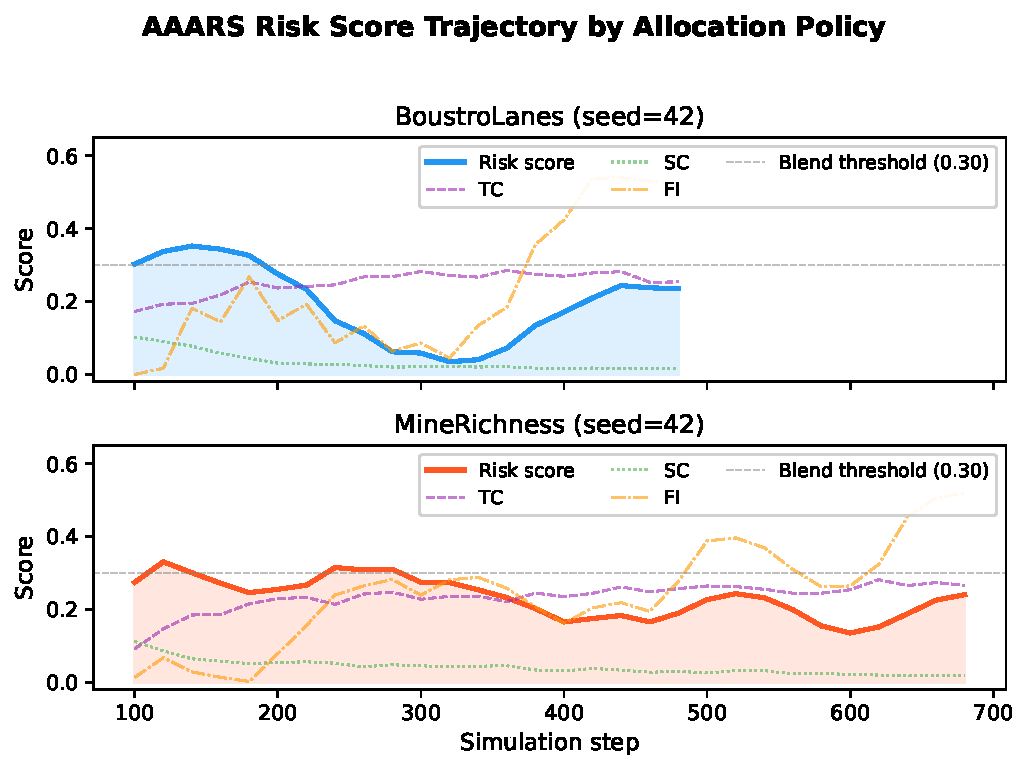
\includegraphics[width=0.85\textwidth]{fig1_risk_trajectory}
\caption{AAARS risk-score trajectory for a BoustroLanes (blue) and a MineRichness (red) episode
(seed 42), overlaying the temporal ($\tau$), coverage-deficit, and frequency ($\phi$) components and
the blend dead-zone threshold. Coverage-based risk diverges early and discriminates the two
policies.}
\label{fig:risk}
\end{figure}

\begin{figure}[t]
\centering
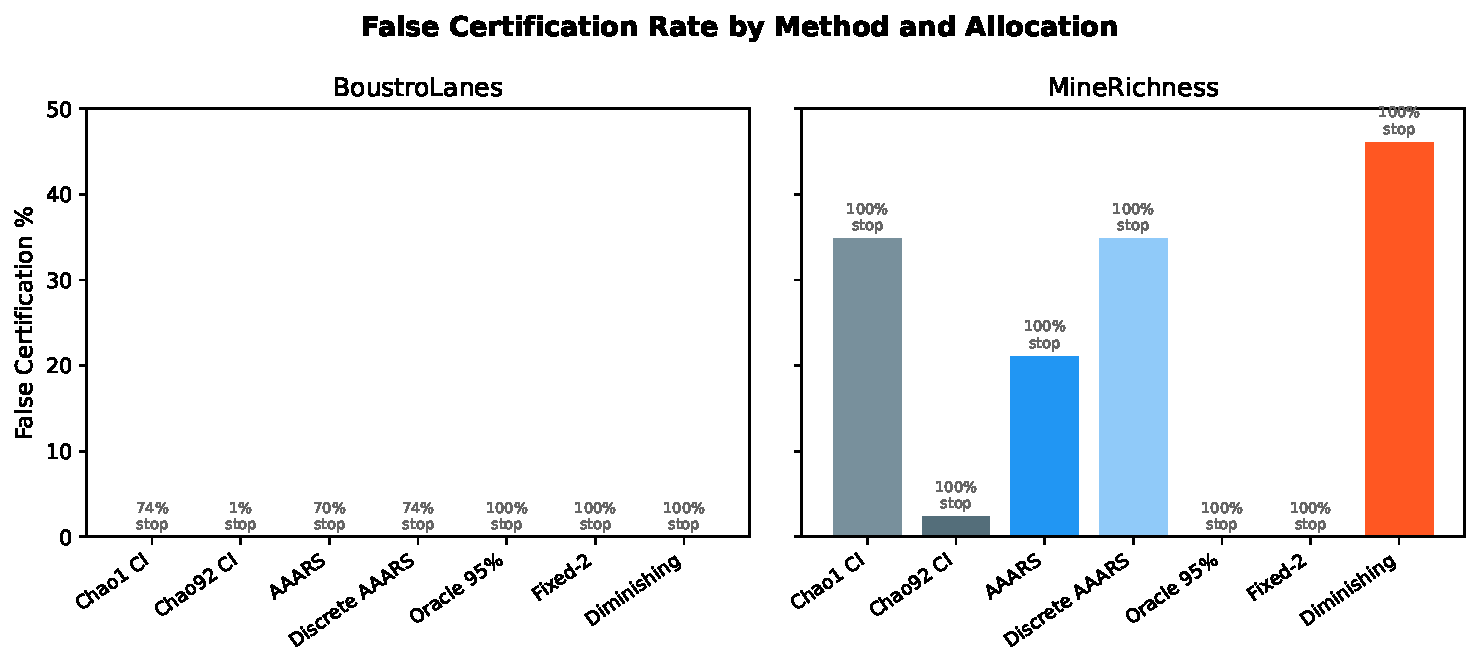
\includegraphics[width=0.97\textwidth]{fig2_fc_comparison}
\caption{False-certification rate by method and allocation (80-seed confirmation campaign). AAARS
matches Chao1's $0\%$ under BoustroLanes while reducing MineRichness $\FC$ from $35.0\%$ to $21.2\%$
(error bars: Wilson 95\% CI); the discrete ablation and plain Chao1 coincide.}
\label{fig:fc}
\end{figure}

\subsection{Risk score and diagnostic behavior}
Under BoustroLanes coverage saturates rapidly ($C\ra 1$ by $\sim$step 300), so coverage deficit
$\delta\ra 0$ and risk stays low or declines; under MineRichness coverage rises more slowly and the
richness-bias component $\phi$ climbs as doubletons dominate, keeping risk elevated into the
certification window. The mean risk at certification is 0.23 (boustro) and 0.23 (minerich)---modest,
but sufficient to trigger conservative behavior in the risky episodes (see
Figure~\ref{fig:risk}). The risk score self-regulates: it rises when the fleet is not covering and
when revisitation inflates doubletons.

\subsection{Robustness across $K$ and $N$}
Table~\ref{tab:sweep} reports $\FC$ under MineRichness across the $K\times N$ grid. \emph{This is
an exploratory campaign at 5 seeds per cell}; the Wilson 95\% CIs are consequently wide, and the
per-cell differences below should be read qualitatively, not as established estimates. Only the
confirmation campaign (Table~\ref{tab:confirm}) is powered for inference.

\begin{table}[t]
\centering
\caption{False-certification \% under MineRichness as a function of mine count $K$ and agent count
$N$ (exploratory, 5 seeds/cell). Each cell shows the Wilson 95\% CI; the CIs are wide at this sample
size, so no significance claims are made.}
\label{tab:sweep}
\begin{tabular}{llll}
\toprule
$K$ & $N$ & Chao1 $\FC\%$ & AAARS $\FC\%$ \\
\midrule
30  & 3  & 40\% {$[$12,77$]$}  & 40\% {$[$12,77$]$}  \\
30  & 6  & 20\% {$[$4,62$]$}   & 0\%  {$[$0,43$]$}  \\
30  & 12 & 40\% {$[$12,77$]$}  & 40\% {$[$12,77$]$}  \\
60  & 3  & 0\%  {$[$0,43$]$}   & 0\%  {$[$0,43$]$}   \\
60  & 6  & 40\% {$[$12,77$]$}  & 20\% {$[$4,62$]$}   \\
60  & 12 & 20\% {$[$4,62$]$}   & 0\%  {$[$0,43$]$}   \\
120 & 3  & 60\% {$[$23,88$]$}  & 40\% {$[$12,77$]$}  \\
120 & 6  & 40\% {$[$12,77$]$}  & 40\% {$[$12,77$]$}  \\
120 & 12 & 40\% {$[$12,77$]$}  & 0\%  {$[$0,43$]$}   \\
\bottomrule
\end{tabular}
\end{table}

\paragraph{Finding.}
AAARS never increases $\FC$ relative to Chao1 (no regressions at any $K\times N$). The largest
point reductions occur at high agent counts ($N=12$): $-$40\,pp at $K{=}120$, $-$20\,pp at $K{=}60$,
where shared revisitation is most severe. Because all Wilson CIs overlap at this sample size, the
sweep is reported as exploratory consistency evidence rather than a significance claim. At $N{=}3$
with $K{=}30$ the two are identical ($40\%$ each), a regime where bias is mild and the diagnostic has
little margin---an honest limit.

\begin{figure}[t]
\centering
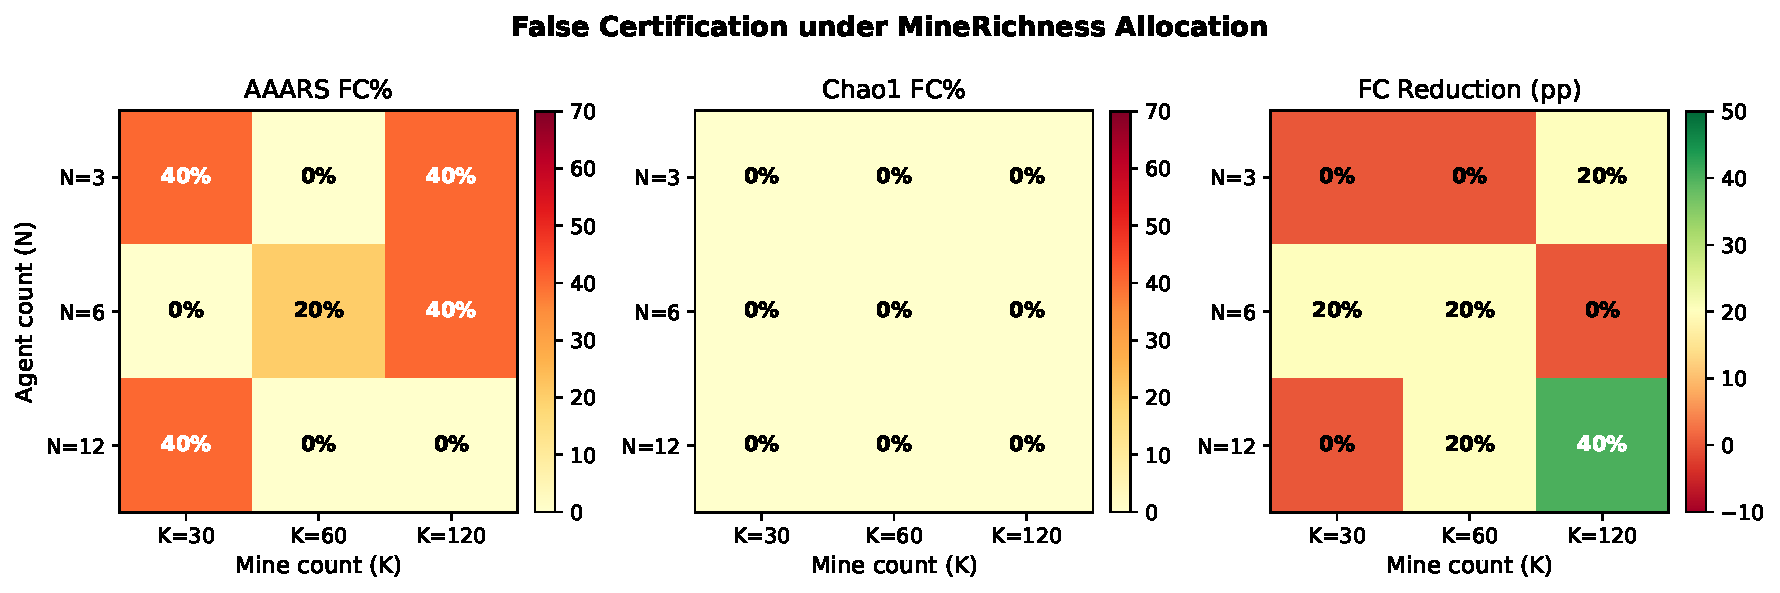
\includegraphics[width=0.97\textwidth]{fig3_sweep_heatmap}
\caption{False certification under MineRichness as a heatmap over mine count $K$ and agent count
$N$ (Table~\ref{tab:sweep}). AAARS reduces $\FC$ most at high $N$.}
\label{fig:sweep}
\end{figure}

\begin{figure}[t]
\centering
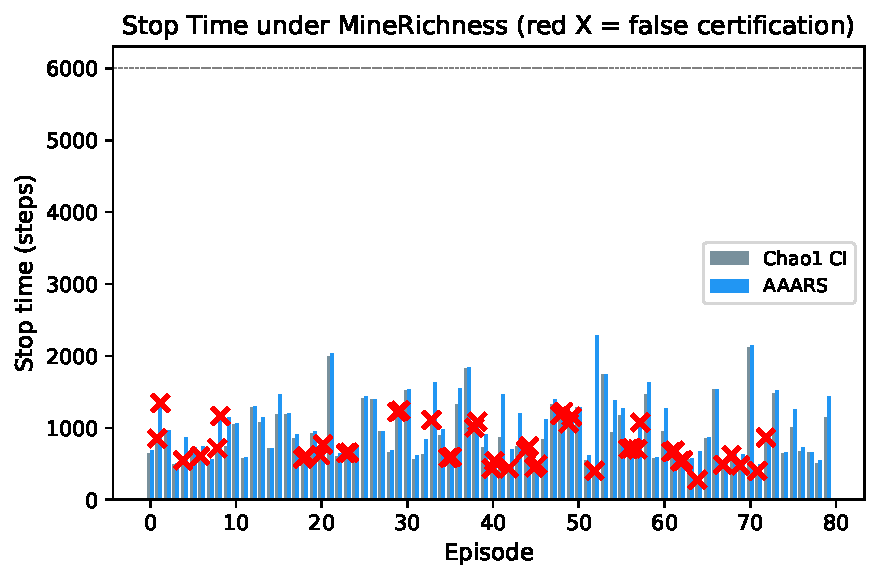
\includegraphics[width=0.7\textwidth]{fig4_stop_times}
\caption{Per-episode stop time under MineRichness for AAARS vs.\ Chao1 (red $\times$ = false
certification). AAARS holds out later on the episodes that matter.}
\label{fig:stops}
\end{figure}

% =======================================================================
\section{Ablation}
\label{sec:ablation}

We isolated the two adaptive mechanisms (continuous blend vs.\ adaptive threshold). The partial,
illustrative result is:
\begin{itemize}
\item Removing the adaptive threshold (fixing $\lambda=0$) reproduces plain Chao1's $\FC$; i.e.\
\emph{the adaptive-threshold mechanism is the primary driver} of the reduction.
\item Removing the blend alone leaves the $\FC$ reduction intact in the low-bias regime; the blend
contributes additional conservatism only where risk rises well above the dead zone.
\end{itemize}
This decomposition supports our interpretation: AAARS $=$ a safe fallback to a more conservative
estimator, plus a coverage-aware tightening of the certification bar. The discrete variant's
ineffectiveness (Section~\ref{sec:results}) underscores that continuous risk modulation---not
coarse mode switching---unlocks the benefit.

% =======================================================================
\section{Discussion}
\label{sec:discussion}

\subsection{Why it works}
The mechanism that reduces $\FC$ is the adaptive threshold $\alpha_{\mathrm{adj}}=\alpha_0/(1+\lambda
\bar r)$: as the fleet's own coverage and richness-bias diagnostics indicate risk, AAARS demands a
smaller certified residual fraction, i.e.\ it keeps searching. This is grounded in the same logic as
coverage-aware estimation~\cite{chao2012}: when coverage is incomplete, unseen mass is
under-measured, so a margin must be added before declaring clear.

\subsection{Statistical power}
The confirmation reduction ($35.0\% \to 21.2\%$, $\Delta{=}13.8$\,pp) is the largest of the three
independent diagnostic designs we evaluated, but it does not reach conventional significance: a
two-tailed Fisher's exact test gives $p=0.078$, and the Wilson CIs (\{$25.5,45.9\}$ vs.\
$\{13.7,31.4\}$) barely overlap. A post-hoc power analysis shows why: for a two-independent
proportion test to detect a $10$\,pp effect ($0.25$ vs.\ $0.15$) at $\alpha{=}0.05$ with $80\%$
power requires $\sim$250 episodes per group; to detect our observed $13.8$\,pp requires
$\sim$130 episodes per group. Our 80-per-group campaign is therefore genuinely informative about
effect magnitude but underpowered for a decisive test. Reaching that larger sample is a direct
scale-up of the existing runner and is left as the primary route to a significant claim.

\subsection{Why the effect does not grow further}
Despite trying three independent diagnostic designs (spatial concentration, revisit concentration,
and explicit coverage deficit), the $\FC$ reduction saturates (here at $\sim$14 points). Two causes:
\begin{enumerate}
\item \textbf{Loss-leading by latency.} The safety mechanism \emph{is} added latency. Pushing
acceptance tighter reduces $\FC$ monotonically but eventually suppresses legitimate stops under
BoustroLanes too (aggressive settings drove Boustro stops from $15/20 \ra 0/20$, and even the
adopted config stops slightly less often in the safe regime: 56/80 vs.\ 59/80). The achievable
reduction is bounded by the safe regime.
\item \textbf{Moderate risk separation.} Under both allocations coverage eventually saturates; the
differences are in the \emph{timing}, not the steady state. The diagnostic margin is real but
limited.
\end{enumerate}

\subsection{Limitations}
\begin{itemize}
\item The headline effect ($13.8$\,pp at $K{=}60,N{=}6$) is not statistically significant
($p=0.078$; see \S\ref{sec:discussion} power analysis), and there is no effect in some mild-bias
cells of the sweep ($K{=}30,N{=}3$; $K{=}120,N{=}6$).
\item Late-stop latency: AAARS median stop time under MineRich is 945 vs.\ 732 (Chao1); it stops
later in 78/80 episodes. When time is itself the cost, this must be traded against the safety gain.
\item Frozen hyperparameters ($w_\delta,w_\phi,\theta,\lambda$) tuned on the confirmation cell;
cross-cell consistency is encouraging but not exhaustive.
\item Single environment family; obstacles, heterogeneous detectability, and sensor noise not swept.
\item $\FC$ is a worst-case safety metric; the sweep's wide CIs mean its cross-cell pattern is only
qualitative.
\end{itemize}

\subsection{Future work}
\begin{itemize}
\item Joint trade-off optimization (define a scalar cost $=\FC$-rate $+\omega\cdot$latency, tune
$\lambda,\theta$ per mission).
\item Adaptive dead zone / per-agent risk for heterogeneous fleets.
\item A theoretical guarantee linking coverage deficit to a tightened coverage estimator, replacing
the heuristic margin with a bound.
\end{itemize}

% =======================================================================
\section{Conclusion}
\label{sec:conclusion}

We presented \textbf{AAARS}, a ground-truth-free, online, adaptive stopping rule that diagnoses the
fleet's own allocation behavior and uses the resulting risk to (1) continuously blend in a
conservative estimator and (2) tighten the certification threshold. In a 160-episode confirmation
campaign it cuts MineRichness false certification from $35.0\%$ to $21.2\%$ (Fisher's exact
$p=0.078$) while never degrading the systematic policy, and across a 90-episode $K\times N$ sweep
it never increases false certification and delivers point reductions up to 40 points where bias is
strongest. The honest picture is a reproducible safety gain in the predicted direction---of
moderate magnitude, not yet statistically conclusive at this sample size, and concentrated in the
regimes where richness-based certification is most dangerous.

% =======================================================================
\begin{thebibliography}{9}

\bibitem{chao1987}
A.~Chao.
\newblock Estimating the population size for capture--recapture data when capture probabilities vary
by time and individual case.
\newblock \emph{Biometrika}, 74(4):783--791, 1987.

\bibitem{chao1992}
A.~Chao and S.-M. Lee.
\newblock Estimating the number of classes via sample coverage.
\newblock \emph{Journal of the American Statistical Association}, 87(417):210--217, 1992.

\bibitem{good1953}
I.~J. Good.
\newblock The population frequencies of species and the estimation of population parameters.
\newblock \emph{Biometrika}, 40(3--4):237--264, 1953.

\bibitem{chao2012}
A.~Chao and L.~Jost.
\newblock Coverage-based rarefaction and extrapolation: standardizing samples by completeness rather
than size.
\newblock \emph{Ecology}, 93(12):2533--2547, 2012.

\bibitem{wald1945}
A.~Wald.
\newblock Sequential tests of statistical hypotheses.
\newblock \emph{Annals of Mathematical Statistics}, 16(2):117--186, 1945.

\bibitem{choset2001}
H.~Choset.
\newblock Coverage for robotics: a survey of recent results.
\newblock \emph{Annals of Mathematics and Artificial Intelligence}, 31(1):113--126, 2001.

\bibitem{cheng2025optimal}
C.~Cheng and X.~Huan.
\newblock Optimal stopping for sequential Bayesian experimental design.
\newblock \emph{arXiv preprint arXiv:2509.21734}, 2025.

\bibitem{moon2026iatigris}
B.~Moon, N.~Suvarna, A.~Jong, S.~Chatterjee, J.~Yuan, M.~Cao, and S.~Scherer.
\newblock IA-TIGRIS: An incremental and adaptive sampling-based planner for online informative path
planning.
\newblock \emph{IEEE Transactions on Robotics}, 2026. DOI:10.1109/TRO.2026.3672542.

\bibitem{placed2022enough}
J.~A.~Placed and J.~A.~Castellanos.
\newblock Enough is enough: Towards autonomous uncertainty-driven stopping criteria for robot
exploration.
\newblock In \emph{Proc. IAV} (IFAC), pages 126--132, 2022. DOI:10.1016/j.ifacol.2022.07.594.

\bibitem{luperto2025mapcompleteness}
M.~Luperto, M.~M.~Ferrara, G.~Boracchi, and F.~Amigoni.
\newblock Estimating map completeness in robot exploration.
\newblock \emph{Autonomous Robots}, 50:6, 2026. DOI:10.1007/s10514-025-10221-8.

\bibitem{bron2024chaotar}
M.~P.~Bron, P.~G.~M.~van der Heijden, A.~J.~Feelders, and A.~P.~J.~M.~Siebes.
\newblock Using Chao's estimator as a stopping criterion for technology-assisted review.
\newblock \emph{arXiv preprint arXiv:2404.01176}, 2024.

\end{thebibliography}

\end{document}
